\section{Exercice 4}
L'objectif de cet exercice est de créer un serveur web répondant aux requêtes HTTP sur un premier port, et renvoyant son fichier de log au client se connectant sur le second port. De nouvelles entrées sont ajoutées dans le fichier de log à chaque fois qu'un client effectue une requête sur le premier port.\\

Deux sockets sont tout d'abord initialisées, \emph{sockfd\_http} et \emph{sockfd\_log} à l'aide de \emph{init\_stream\_ server\_socket()} sur deux ports différents.\\

On souhaite ensuite effectuer un traitement différent si les requêtes sont reçues sur la première ou la seconde socket. Pour cela, les forks ou encore les threads auraient pu être utilisés. Une solution plus simple utilisant la fonction \emph{select()} a cependant été retenue. Cette fonction prend en paramètre des sets de descripteurs de fichiers : \emph{readfds}, \emph{writefds} et \emph{exceptfds}. Celui qui nous intéresse est \emph{readfds}, celui-ci étant modifié lorsque \emph{select()} est exécuté pour indiquer quels descripteurs de fichiers ont des données qui peuvent être lues.\\

\begin{mdframed}[backgroundcolor=lightblue, linecolor=darkblue]
Sachant que les sets passés en paramètre à \emph{select()} sont modifiés à chaque exécution, deux sets sont créés : \emph{master} et \emph{readfds}. A chaque itération de la boucle principale, \emph{master} est copié dans \emph{readfds}, et ce dernier est passé en paramètre de \emph{select()}.

\begin{mdframed}[backgroundcolor=lightblue2, linecolor=darkblue]
\textbf{select(2) man page :}\\
``On exit, the sets are modified in place to indicate which file descriptors actually changed status.''
\end{mdframed}
\end{mdframed}
\

S'il y a des données qui peuvent être lues sur la première socket (\emph{sockfd\_http}), alors on accepte la connexion du client à la socket (\emph{accept()}) puis on traite la requête avec la fonction \emph{handle\_GET\_request()}. Celle-ci fait appel à \emph{recv\_res\_GET\_request} (fichier \emph{http\_tools.c}) qui permet de recevoir une requête HTTP et la parser afin de récupérer le chemin de la ressource que souhaite obtenir le client. Une ligne est ensuite ajoutée dans le fichier de log au format \emph{adresse du client - date - ressource souhaitée} à l'aide de \emph{log\_line()}. Enfin, le fichier est envoyé à l'aide de la fonction \emph{sendfile\_HTTP\_helper()} (fichier http\_tools.c).\\

\begin{lstlisting}
int handle_GET_request(int clientfd, struct in_addr client_addr) {
    int status;
    char *path, *res;

    // Retrieve resource
    res = recv_res_GET_request(clientfd);
    if (res == NULL) {
        return -1;
    }

    log_line(client_addr, res);

    if (strcmp(res, "/") == 0) {
        path = DEFAULT_PAGE;
    }
    else {
        path = res + 1; // file path without the leading "/"
    }

    status = sendfile_HTTP_helper(path, clientfd);

    free(res);

    return status;
}
\end{lstlisting}
\

La fonction \emph{sendfile\_HTTP\_helper()} ouvre le fichier demandé, puis envoi une réponse 404 (NOT FOUND) si l'ouverture échoue. Si l'ouverture s'effectue correctement, on envoi une réponse 200 (OK) suivie de l'envoi du fichier avec \emph{fsendfile\_helper()} (fichier file\_tools.c).\\

\begin{lstlisting}
int sendfile_HTTP_helper(char* filepath, int fd_dest) {
    int filefd, status;
    char *content_type, *response;

    /* retrieve the content_type with the file extension (unsafe, but probably
     * sufficient for this exercise). */
    if (strstr(filepath, ".html") != NULL) {
        content_type = TYPE_HTML;
    }
    else if(strstr(filepath, ".txt") != NULL) {
        content_type = TYPE_PLAIN_TEXT;
    } else {
        content_type = TYPE_OCTET_STREAM;
    }

    // Open requested file
    filefd = open(filepath, O_RDONLY);
    if (filefd == -1) {
        perror("open");

        // file not found -> HTTP 404 response
        if (errno == ENOENT) {
            send_complete(fd_dest, HTTP_404_RESPONSE, strlen(HTTP_404_RESPONSE));
        }

        return -1;
    }

    // HTTP 200 response
    response = create_HTTP_200_response(content_type);
    if (response == NULL) {
        close(filefd);
        return -1;
    }

    // Send the HTTP response to the client
    status = send_complete(fd_dest, response, strlen(response));
    free(response);
    if (status == -1) {
        close(filefd);
        return -1;
    }

    // send requested file
    status = fsendfile_helper(filefd, fd_dest);

    close(filefd);

    return status;
}
\end{lstlisting}
\

Si des données peuvent être lues sur la seconde socket (\emph{sockfd\_log}), on accepte également la connexion du client, et on envoi le fichier de log avec la fonction \emph{sendfile\_HTTP\_helper()} décrite précédemment.

\newpage
\subsection{Exemple d'exécution}

\begin{figure}[h!]
	\centering
	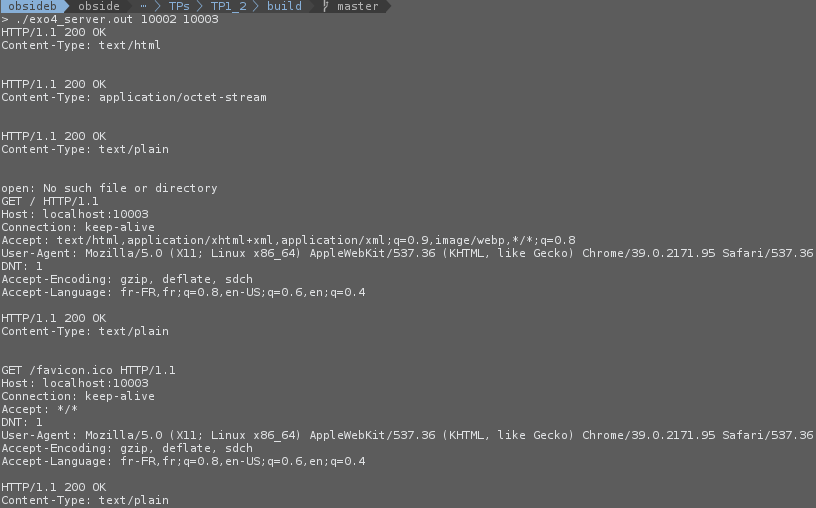
\includegraphics[width=0.9\textwidth]{screenshots/ex4_terminal.png}
	\caption{exo4\_server.out - terminal}
\end{figure}

\begin{figure}[h!]
        \centering
        \begin{subfigure}[b]{0.32\textwidth}
                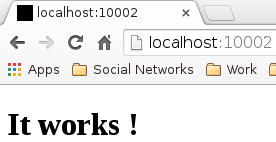
\includegraphics[width=\textwidth]{screenshots/ex4_chrome_index.png}
                \caption{navigateur - index.html}
                \label{fig:ex5_index}
        \end{subfigure}%
        ~
        \begin{subfigure}[b]{0.32\textwidth}
                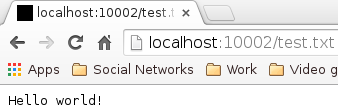
\includegraphics[width=\textwidth]{screenshots/ex4_chrome_test.png}
                \caption{navigateur - test.txt}
                \label{fig:ex5_test}
        \end{subfigure}
        ~
        \begin{subfigure}[b]{0.32\textwidth}
                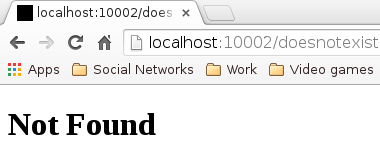
\includegraphics[width=\textwidth]{screenshots/ex4_chrome_doesnotexist.png}
 	            \caption{navigateur - fichier non existant}
                \label{fig:ex5_doesnotexist}
        \end{subfigure}
        \caption{navigateur - requêtes sur le premier port}
\end{figure}

\begin{figure}[h!]
	\centering
	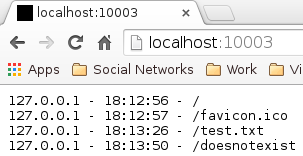
\includegraphics[width=0.4\textwidth]{screenshots/ex4_chrome_log.png}
	\caption{navigateur - requête sur le second port : log}
\end{figure}
